\section{Étude préalable}
\subsection{Étude de l'existant}

\subsubsection{L'état du matériel}
L'état du matériel est l'un des parties importantes dans le POS monitoring pour connaitre les états des composants matériels des TPE :
\begin{itemize}[label=\textbullet]
\item  Lecteur de cartes
\item  Lecteur de cartes à puce
\item  Stockage
\item  RAM
\item  Processeur
\item  Batterie
\item  Pin pad
\item  Connexion
\item  Ancre
\item  imprimante
\item  papiers
\item  ...
\end{itemize}


A tous moments où le commerçant veut savoir l'état du matériel d'un TPE ou d'un groupe des TPE, il peut demander tous les informations qu'il veut.\\

\subsubsection{L'état du logiciel}
Cette partie représente tous Types d'informations sur l'état logiciel d'un TPE ou groupe des TPE.
\begin{itemize}[label=\textbullet]
\item  Paramètres 
\item  Cryptographie
\item  ...
\end{itemize}

A tous moments où le commerçant veut savoir l'état du logiciel d'un TPE ou d'un groupe des TPE, il peut demander tous les informations qu'il veut.\\


\subsubsection{Reportings}
La partie reporting ou statistique et la deuxième partie du POS monitoring, cette partie est très importante pour les utilisateurs des TPE pour savoir tous types importants d'informations au niveau financière.\\

L’ensemble des reportings sont élaborés sur la base des informations suivantes :
\begin{itemize}[label=\textbullet]
\item Nombre de transactions 
\item Nombre de transactions rejetées
\item Cause de rejet 
\item Types des réseaux( visa,mastercard...)
\item Type d'activité du commerçant
\item ...
\end{itemize}


A tous moments le commerçant peut voir l'ensemble des statistiques d'un TPE ou d'un groupe des TPE, soit présentées par chiffres ou par des graphes.\\

\begin{figure}[h!]  
  %\centering
   % 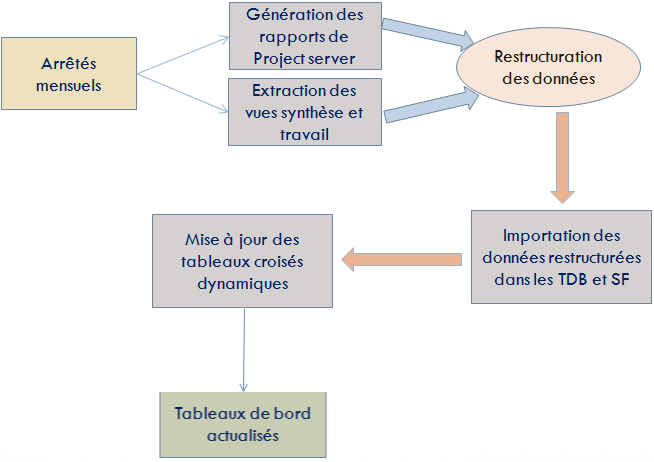
\includegraphics[width=1\textwidth]{chapitre2/Figures/process.png}
 % \caption{Processus de génération des tableaux de bord}
\end{figure}


\subsubsection*{Exemple de Reportings :}
La partie suivante comporte un exemples de reportings actuels générés à partir des tableaux croisés dynamiques d’Excel, accompagnés d’explications.

\begin{figure}[h!]  
  \centering
    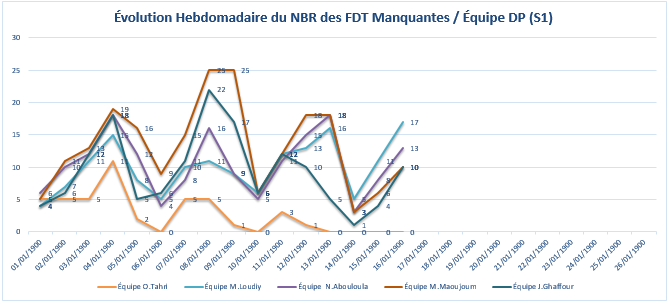
\includegraphics[width=1\textwidth]{chapitre2/Figures/exemple1.png}
  \caption{Tableau de bord suivi FDT}
\end{figure}
Ce rapport est un exemple qui ilustre le suivi des FDT manquantes pour chaque Directeur de projet.




\subsection{Critique de l’existant}
Les responsables ont besoin des reportings qui synthétisent des indicateurs sur les ressources, les gains, la situation de la production globale et la situation des projets pour mettre en place les actions nécessaires.\\
L’élaboration des reportings est confiée au POS monitoring, sauf qu’elle représente pour lui une tache répétitive et qui nécessite une charge considérable pour préparer, mettre à jour et présenter les indicateurs dans les délais :
\begin{itemize}[label=\textbullet]
\item La restructuration des rapports et des vues extraits à partir de Project server :
\begin{itemize}
\item Suppression des données inutiles et retenue des informations de l’agence
\item Ajout de nouvelles colonnes pour afficher d’autres indicateurs
\item Conversion des données dans les rapports extraits
\end{itemize}
\item L’import des données de ces rapports vers les tableaux de bord
\item La préparation des données à travers les fonctions Excel (RechercheV, calculs, comparaison, vérification) ce qui peut engendrer des erreurs de calculs et de vérifications
\item L’actualisation de tous les tableaux croisés dynamiques
\item La vérification de la cohérence des indicateurs affichés dans les tableaux et dans les graphes prédéfinis
\item Saisie manuelle des données pour quelques rapports (ressources et indicateurs RH, suivi des feuilles de temps)
\end{itemize}
Le PMO cherche toujours à améliorer et créer des nouveaux rapports pour mettre à disposition des responsables, des indicateurs pertinents, répondant à leurs besoins de suivis.\\
Le PMO est obligé de réinitialiser chaque début d’année, tous les tableaux de bord et le suivi financier pour garder juste les indicateurs de l’année.
\subsubsection*{Communication des indicateurs}
Après l’élaboration des reportings, le PMO doit informer et présenter à l’ensemble des responsables les indicateurs générés.\\
Vu que le PMO est la seule personne qui consolide et centralise l’ensemble des indicateurs, sa présence s’avère indispensable, surtout pour répondre aux nouvelles demandes des responsables, vu qu’ils sont souvent contraints à une mobilité géographique.
